\section{Date: 2026-11-28}
\noindent \textbf{Series ID: TUVPCPIPCPPPT} 

\noindent This series is titled Prices: Consumer Price Index for Tuvalu and has a frequency of Annual. The units are Percent Change and the seasonal adjustment is Not Seasonally Adjusted.The observation start date is 2001-01-01 and the observation end date is 2031-01-01.The popularity of this series is 3. \\ 

\noindent \textbf{Series ID: UOCDSA156MSFRBNY} 

\noindent This series is titled Current Unfilled Orders; Percent Reporting Decreases for New York and has a frequency of Monthly. The units are Percent and the seasonal adjustment is Seasonally Adjusted.The observation start date is 2001-07-01 and the observation end date is 2026-11-01.The popularity of this series is 1. \\ 

\subsection{Raw Regression}
\noindent Regresses the two series against each other directly. A significant result here can come just as easily from both series sharing a long-run trend as from any real relationship.

\begin{center}
\begin{tabular}{lclc}
\toprule
\textbf{Dep. Variable:}             & value\_fred\_UOCDSA156MSFRBNY & \textbf{  R-squared:         } &     0.110   \\
\textbf{Model:}                     &              OLS              & \textbf{  Adj. R-squared:    } &     0.072   \\
\textbf{Method:}                    &         Least Squares         & \textbf{  F-statistic:       } &     2.850   \\
\textbf{Date:}                      &        Sat, 28 Nov 2026       & \textbf{  Prob (F-statistic):} &    0.105    \\
\textbf{Time:}                      &            19:12:35           & \textbf{  Log-Likelihood:    } &   -74.605   \\
\textbf{No. Observations:}          &                 25            & \textbf{  AIC:               } &     153.2   \\
\textbf{Df Residuals:}              &                 23            & \textbf{  BIC:               } &     155.6   \\
\textbf{Df Model:}                  &                  1            & \textbf{                     } &             \\
\textbf{Covariance Type:}           &           nonrobust           & \textbf{                     } &             \\
\bottomrule
\end{tabular}
\begin{tabular}{lcccccc}
                                    & \textbf{coef} & \textbf{std err} & \textbf{t} & \textbf{P$> |$t$|$} & \textbf{[0.025} & \textbf{0.975]}  \\
\midrule
\textbf{const}                      &      22.1982  &        1.298     &    17.101  &         0.000        &       19.513    &       24.883     \\
\textbf{value\_fred\_TUVPCPIPCPPPT} &      -0.4180  &        0.248     &    -1.688  &         0.105        &       -0.930    &        0.094     \\
\bottomrule
\end{tabular}
\begin{tabular}{lclc}
\textbf{Omnibus:}       &  1.017 & \textbf{  Durbin-Watson:     } &    2.196  \\
\textbf{Prob(Omnibus):} &  0.602 & \textbf{  Jarque-Bera (JB):  } &    0.572  \\
\textbf{Skew:}          & -0.369 & \textbf{  Prob(JB):          } &    0.751  \\
\textbf{Kurtosis:}      &  2.943 & \textbf{  Cond. No.          } &     6.93  \\
\bottomrule
\end{tabular}
%\caption{OLS Regression Results}
\end{center}

Notes: \newline
 [1] Standard Errors assume that the covariance matrix of the errors is correctly specified.

\begin{figure}
\centering
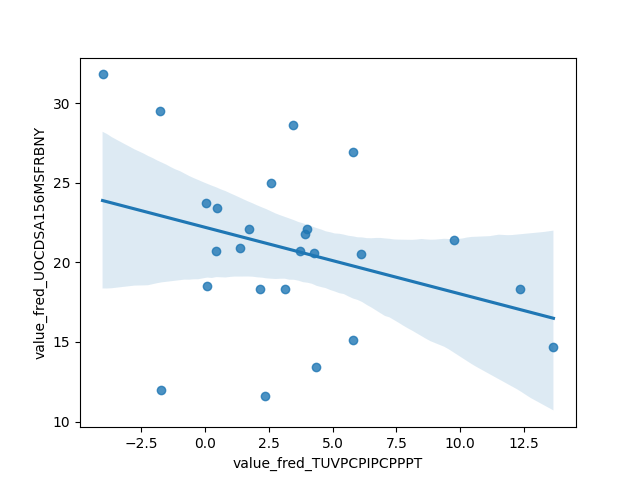
\includegraphics[scale = 0.9]{plots/plot_2026-11-28.png}
\caption{Raw Regression Plot for 2026-11-28}
\end{figure}
\newpage
\subsection{Detrended Regression}
\noindent Regresses the residuals of each series after removing its own linear time trend, so a shared trend can no longer drive the result on its own. A relationship that stays significant here is better evidence of a genuine link between the two series.

\begin{center}
\begin{tabular}{lclc}
\toprule
\textbf{Dep. Variable:}                        & value\_fred\_UOCDSA156MSFRBNY\_detrended & \textbf{  R-squared:         } &     0.100   \\
\textbf{Model:}                                &                   OLS                    & \textbf{  Adj. R-squared:    } &     0.061   \\
\textbf{Method:}                               &              Least Squares               & \textbf{  F-statistic:       } &     2.556   \\
\textbf{Date:}                                 &             Sat, 28 Nov 2026             & \textbf{  Prob (F-statistic):} &    0.124    \\
\textbf{Time:}                                 &                 19:12:35                 & \textbf{  Log-Likelihood:    } &   -74.515   \\
\textbf{No. Observations:}                     &                      25                  & \textbf{  AIC:               } &     153.0   \\
\textbf{Df Residuals:}                         &                      23                  & \textbf{  BIC:               } &     155.5   \\
\textbf{Df Model:}                             &                       1                  & \textbf{                     } &             \\
\textbf{Covariance Type:}                      &                nonrobust                 & \textbf{                     } &             \\
\bottomrule
\end{tabular}
\begin{tabular}{lcccccc}
                                               & \textbf{coef} & \textbf{std err} & \textbf{t} & \textbf{P$> |$t$|$} & \textbf{[0.025} & \textbf{0.975]}  \\
\midrule
\textbf{const}                                 &   -2.616e-13  &        0.994     & -2.63e-13  &         1.000        &       -2.056    &        2.056     \\
\textbf{value\_fred\_TUVPCPIPCPPPT\_detrended} &      -0.4004  &        0.250     &    -1.599  &         0.124        &       -0.919    &        0.118     \\
\bottomrule
\end{tabular}
\begin{tabular}{lclc}
\textbf{Omnibus:}       &  0.912 & \textbf{  Durbin-Watson:     } &    2.223  \\
\textbf{Prob(Omnibus):} &  0.634 & \textbf{  Jarque-Bera (JB):  } &    0.419  \\
\textbf{Skew:}          & -0.317 & \textbf{  Prob(JB):          } &    0.811  \\
\textbf{Kurtosis:}      &  3.015 & \textbf{  Cond. No.          } &     3.97  \\
\bottomrule
\end{tabular}
%\caption{OLS Regression Results}
\end{center}

Notes: \newline
 [1] Standard Errors assume that the covariance matrix of the errors is correctly specified.

\begin{figure}
\centering
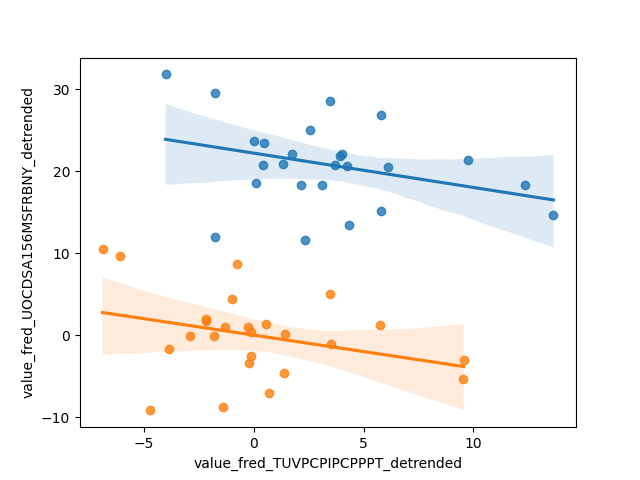
\includegraphics[scale = 0.9]{plots/plot_2026-11-28_detrended.png}
\caption{Detrended Regression Plot for 2026-11-28}
\end{figure}
\newpage
